\documentclass[conference]{IEEEtran}

\usepackage{amsmath}
\usepackage{algorithm}
\usepackage{algpseudocode}
\usepackage{graphicx}
\usepackage{tipa}

\makeatletter
\def\BState{\State\hskip-\ALG@thistlm}
\makeatother

\newcommand{\argmax}{\arg\!\max}

% correct bad hyphenation here
\hyphenation{op-tical net-works semi-conduc-tor}

\begin{document}

\title{Analyzing Differences in Indonesian Spontaneous and Dictated Speech}

\author {
    \IEEEauthorblockN {
        Cil Hardianto Satriawan\IEEEauthorrefmark{1},
        Dessi Puji Lestarti\IEEEauthorrefmark{2}
    }
    \IEEEauthorblockA {
        School of Electrical Engineering and Informatics\\
        Bandung Institute of Technology\\
        Bandung, Indonesia 40132\\
        \IEEEauthorrefmark{1}23515053@std.stei.itb.ac.id,
        \IEEEauthorrefmark{2}dessi@informatika.org
    }
}

\maketitle

\begin{abstract}
The accurate recognition of spontaneous speech is crucial in achieving practical speech recognition.
Statistical-based recognition models typically employ a large amount of read or dictated speech for training, which often yields poor spontaneous recognition performance.
Many approaches have been forwarded to improve performance, including model adaptation and model switching.
In an effort to improve Indonesian language spontaneous recognition performance, we attempt to pinpoint the acoustic differences between spontaneous and dictated Indonesian speech.
At the phoneme level, we find that there are differences in the distribution and pronunciation of several key phonemes associated with filled pauses.
Across speakers, there is a consistent reduction in segment duration and segment energy, with a less marked spectral reduction.
Using these differences as a starting point, we train an SVM that classifies spontaneous and read Indonenesian utterances at 75\% and 87\% accuracy, respectively.
We show that it is possible to obtain this classification by considering segment acoustic features and differences between consecutive segments.
\end{abstract}

\begin{IEEEkeywords}
speech recognition,
\end{IEEEkeywords}

\IEEEpeerreviewmaketitle

\section{Introduction}
The ability to accurately recognize spontaneous speech is a significant hurdle to the practical use of a speech recognition system, with many systems performing poorly.
This is seemingly in contrast to the recognition performance achievable on most state-of-the-art statistical-based systems on dictated speech tasks and limited domain spoken interactions.
In \cite{hoesen}, an Indonesian language speech recognition system was built that is capable of achieving upwards of 80\% accuracy for dictated speech but only around 65\% for spontaneous speech.
Other examples can be found in \cite{}, \cite{}, and \cite{}.

This poor performance may be partly attributed to the fact that a large proportion of the data used to train models is derived from dictated instead of spontaneous speech.
Recording and labelling large amounts of new spontaneous speech is a difficult and costly process, whereas existing Indonesian language resources are scarce or non-existant.
In addition, although spontaneous recognition is an important component of practical speech recognition, research has only relatively recently shifted in this direction.

Spontaneous and dictated speech also differ in various ways.
It has been proposed that spontaneous speech is less ordered both linguistically and acoustically \cite{nakamura1}, and differs spectraclly from dictated speech \cite{nakamura2}.
Spontaneous speech contains filled pauses, repairs, hesitations, repetitions, and disfluencies, which are largely absent in dictated speech.
The exact differences vary by language, with some languages exhibiting a strong tonal difference between spontaneous and dictated speech \cite{spanish}\cite{dwello}.
Speech disfluencies also differ between language and speaker; each language, dialect, or speaker may have their own set of specific disfluencies and patterns.

A number of methods have been developed to improve spontaneous speech recognition performance.
In the model adaptation approach, a large amount of dictation data is adapted to a small amount of spontaneous data while training the acoustic model, using a method such as Maximum A Priori (MAP).
In the second approach, acoustic and language models for spontaneous and dictated speech are trained separately, with a method to switch or weigh models on the fly.
Model switching relies on a reliable way to differentiate between spontaneous and dictated speech that is independent of the specific acoustic models.

In either case, it is instructive to understand how acoustic differences between spontaneous and dictated speech manifest and how to describe them.
With a better understanding of these differences we can train better specialized models for spontaneous or mixed speech, for example utilizing the model switching approach.
The goal is to achieve a reasonably performant "front-end" classifier that can pass data to a number of back-end models specialized for the task at hand.

In the following sections we describe the relevant literaturea and the speech corpus used for analysis.
We then discuss at length the various phoneme-level differences between spontaneous and read speech in the Indonesian language.
Finally we attempt to engineer segment-level acoustic features and utilize this feature set to classify segmented utterances.

\section{Related Works}

Furui has shown that there is a substantial difference in the spectral properties of vowels between read and spontaneous speech \cite{furui1}.
In this approach, differences between phoneme vectors of varying styles and their centers are compared using the following formulation:

This can be interpreted
In this approach, MFCC features are taken

The literature suggests that many spontaneous speech 

Wang, et al. \cite{wang} proposed an incremental ensemble method called Accuracy-Weighted Ensembles (AWE).
It is a weighted majority ensemble algorithm with the weight is calculated based on error reduction analysis.
Each classifier $c_i$ is given a weight reversely proportional to the expected error MSE$_i$.
The weight is then calculated as $w_i = \text{MSE}_i - \text{MSE}_r$ where $\text{MSE}_r$ is the mean square error of a random classifier.

AWE proposed by Wang, et al. \cite{wang} is used as ensemble method for our approach.
Its weighting method is based on expected error of classifier.
We compute the mean square error of classifier $c_i$ by using formula
\[\text{MSE}_i = \frac{1}{|S|} \sum_{(x,y) \in S} (1 - f_i^y(x))^2\]
where $S$ is the latest chunk of training data, $(x,y)$ is a record in $S$ with $y$ is the true label, and $f_i^y(x)$ is the probability given by $c_i$ that $x$ is an instance of label $y$.
And then, the mean square error of each label according to its distribution is
\[\text{MSE}_r = \sum_{c} p(c)(1-p(c))^2\]
Finally, the weight $w_i$ of a classifier $c_i$ is computed with formula
\[w_i = \text{MSE}_r - \text{MSE}_i\]
$\text{MSE}_r$ does not contain useful information about the data.
It is only used as a threshold to discard classifiers from ensemble.
We eliminate classifiers that have negative weight, which means their error is equal or larger than $\text{MSE}_r$.

Another ensemble method for incremental learning is Streaming Ensemble Algorithm (SEA) \cite{street}.
It combines decision tree models using majority-voting.
It does not weight each classifier and vote accordingly.
It is based on investigation that weighting had little or no effect on ensemble accuracy.

Both ensemble methods are applied on concept drifting environment.
We concluded that concept drift has the same meaning as what we called OOV condition in the sense of the underlying concept, which we considered as terms or words, does not reflected in the predictive features \cite{street}.
The concept can also change without warning.
Zang, et al. \cite{zang} shows that AWE performs better than SEA.

For multilabel classification task, there are two main approach: problem transformation and algorithm adaptation \cite{tsoumakas}.
In problem transormation approach, some commonly methods are Binary Relevance (BR), Label Powerset (LP), and Calibrated Label Ranking (CLR).
Some examples of algoritm adaptation methods are Adaboost.MH, Adaboost.MR, and MLkNN.

In BR, multilabel dataset is transformed into $n$ single-label dataset where $n$ is the number of label \cite{prajapati}.
CLR applies the comparisons among the pair of labels exist in dataset, then builds both pair and single-label models.
LP method changes multilabel classification into a multiclass classification \cite{demb} by adding some new single-labels for each unique set of labels exists in multilabel dataset \cite{prajapati}.

The first two methods of algorithm adaptation are the extension of AdaBoost algorithm that search for accurate classification rules by combining multiple weak hypothesis \cite{dharmadhikari}.
MLkNN is the adaptation of kNN algorithm which uses kNN separately for each label then determines the k closest instances to the tested one.
Adaboost.MH and Adaboost.MR perform well in terms of one error, coverage, ranking loss and average precision, while MLkNN performs better in terms of hamming loss \cite{zhang}.

\section{Speech Corpus}

The Perisalah Corpus is a collection of spontaneous and read speech recorded for the development of the Perisalah Speech Recognition System \cite{} in collaboration with PT. Inti, an Indonesian public telecommunications company.
The corpus samples a variety of different age groups and local dialects.
The meeting transcription system is being deployed at various government institutions at the national and regional levels.
The read/dictation part of the corpus was build to be lexically balanced with respect to written Indonesian.

\subsection{Corpus Overview}

After cleaning, the corpus consists of 297 native Indonesian speakers, with on average 275 dictated and 61 spontaneous utterances per speaker, totalling 81240 dictated and 18210 spontaneous utterances, respectively.
On average, dictated utterances are 6.54 seconds long and spontaneous utterances 8.33 seconds long for a total of 147.6 and 42.1 hours of dictated and spontaneous speech, respectively.

Demographically, speakers were taken from both genders roughly equally, with 143 male speakers and 154 female speakers.
Fig. \ref{demographics1} shows the distribution of genders across dialects, the sampled dialects being Javanese (J), Sundanese (S), Minanga (M), Batak (T), Betawi/Melayu (A), Balinese (B), Sulawesi (W), and Maluku/Papua (P).
Roughly 57\% of Indonesians live on Java, where the Javanese, Sundanese, and Betawi/Melayu dialects originate.
Two age groups were defined; ages 40 years and under, and ages above 40 years, with 243 and 53 speakers, respectively.

\begin{figure}[!htb]
\centering
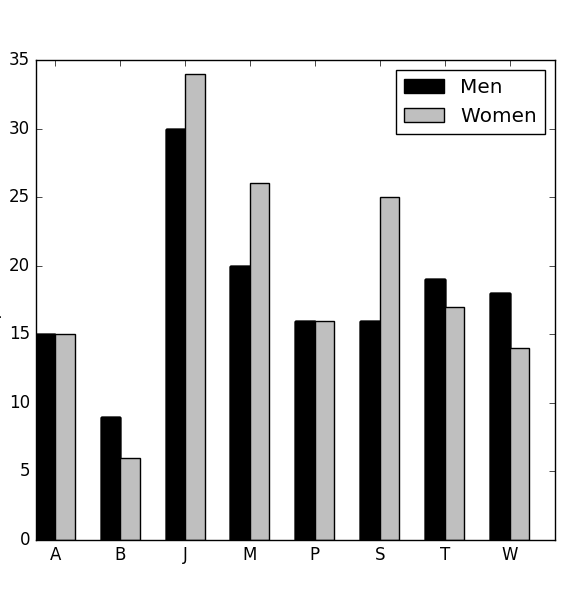
\includegraphics[width=3.0in]{demographics1_bw}
\caption{Number of members of each gender for each dialect}
\label{demographics1}
\end{figure}

Utterances for prepared texts were taken from newspaper articles and magazines, and hence derived from real-world examples, albeit written ones.
A total of ten different sets were compiled, labelled from 'A' to 'J'.
Speakers were recorded in a single session, with read speech recorded first and spontaneous speech afterwards.
For spontaneous speech, speakers were asked to choose an arbitrary topic in which they were comfortable with and thus asked to speak at length about it.

Fluency of speech varies greatly within the corpus, with some participants experiencing difficulties reading fluently, while others were highly uncomfortable when told to improvise a topic.
Utterances for spontaneous speech were segmented by hand; that is, the start and end of sentences is dependent on the studio operator's comprehension of the speech, although supervision was provided.
Hence, using the duration of utterances as a metric should be done with caution.

\subsection{Acoustic feature extraction}

Speech audio data is represented as audio samples taken at a particular rate.
A constant number of (overlapping) audio samples are processed in a frame to obtain low level spectral, cepstral, and energy features.
A segment, comprised of a varying number of such frames, represents a single phoneme.
For the purposes of our acoustic analysis, linguistic units other than the phoneme are ignored and we instead consider utterances as sequences of segments.
In addition to frame and segment-level acoustic information a number of high level features are obtained at the utterance and speaker levels, namely the specific speaker of an utterance, their gender, dialect, and age.

Using segments as the smallest unit of analysis is attractive and practical for many reasons.
Analysis of individual frames is impractical on very large datasets due to the computational load.
In addition, as we shall see, utilizing sequences of segments leads to usable spontaneous/read classification results at a relatively low latency and computational/memory overhead.
On the other hand, the identification of segment boundaries is usually accomplished by first training a HMM.

In order to obtain training data segments, forced alignment was conducted on the corpus using a pretrained HMM built using the Kaldi toolkit.
The segment duration and location in the utterance in seconds and phone was obtained for each utterance in the corpus.
171 phones were defined including fillers, silence, and other non-speech phones.
The 64 most common phones calculated by frequency of appearance in the corpus are displayed in Table \ref{phones}.
These phones account for 98.15\% of the segment occurences in the corpus.
Voiced phones are further separated as belonging to the beginning, inside, or end of a word, indicated by a 'B', 'I', and 'E' suffix, resepectively.
The '@' symbol represents the phonetic '\textipa{@}'.

\begin{table}[!htb]
\renewcommand{\arraystretch}{1.3}
\caption{Common phones}
\label{phones}
\centering
\begin{tabular}{|c|c|c|c|c|c|c|c|}
    \hline
    @\_B & @\_E & @\_I & a\_B & a\_E & a\_I & b\_B & b\_I\\
    \hline
    c\_B & c\_I & d\_B & d\_I & e\_B & e\_I & f\_B & f\_I\\
    \hline
    g\_B & g\_I & h\_B & h\_E & h\_I & i\_B & i\_E & i\_I\\
    \hline
    j\_B & j\_I & k\_B & k\_E & k\_I & l\_B & l\_E & l\_I\\
    \hline
    m\_B & m\_E & m\_I & n\_B & n\_E & n\_I & ng\_E & ng\_I\\
    \hline
    ny\_I & o\_B & o\_E & o\_I & p\_B & p\_E & p\_I & r\_B\\
    \hline
    r\_E & r\_I & s\_B & s\_E & s\_I & sil & t\_B & t\_E\\
    \hline
    t\_I & u\_B & u\_E & u\_I & w\_B & w\_I & y\_B & y\_I\\
    \hline
\end{tabular}
\end{table}

Utilizing alignment information regarding duration and location of segments, frame features were generated or inserted, frames aligned to the correct semgent, and then averaged for each segment.
The segment features obtained this way are segment-averaged formants (generated) and MFCCs (inserted).
The first four formants of each frame were calculated by solving the Linear Predictive Coefficients (LPC) of each frame in the frame alignment subroutine.
The first 13 MFCCs were obtained during the pretraining of the segmentation HMM through the Kaldi toolkit, using the training defaults including Cepstral Mean Subtraction (CMS).
The delta and delta-delta features were calculated manually during frame alignment.
Apart from averaged frames, features at the segment level include segmental duration and location, and segment label in terms of phoneme. 
The complete list of features is shown in Table \ref{features}.

\begin{table}[!htb]
\renewcommand{\arraystretch}{1.3}
\caption{Acoustic features}
\label{features}
\centering
\begin{tabular}{|l|r|r|r|r|r|}
    \multicolumn{1}{c}{} \textbf{Segment-level features}\\
    \hline
    Cepstral (36) & MFCC 12 + $\Delta$12 + $\Delta\Delta$12\\
    \hline
    Log energy (3) & MFCC 1 + 1$\Delta$ + 1$\Delta\Delta$\\
    \hline
    Temporal (2) & Duration 1 + Position 1\\
    \hline
    Spectral (4) & Formants 4 F0 - F4\\
    \hline
    \multicolumn{1}{c}{} \textbf{Utterance-level features}\\
    \hline
    Utterance ID (1) & Utterance number\\
    \hline
    Label (1) & Spontaneous or dictated\\
    & 'Z' for spontaneous or\\
    & one of 'A' - 'J' for dictated\\
    \hline
    \multicolumn{1}{c}{} \textbf{Speaker-level features}\\
    \hline
    Speaker ID (1) & Speaker number\\
    \hline
    Gender (1) & Female or male\\
    \hline
    Dialect (1) & Jawa (J), Sunda (S)\\
    & Minang (M), Batak (T)\\
    & Betawi/Melayu (A)\\
    & Bali (B), Sulawesi (W)\\
    & or Maluku/Papua (P)\\
    \hline
    Age group (1) & Young (M) or old (L)\\
    \hline
\end{tabular}
\end{table}

\subsection{Phone analysis}

The analysis of data that follows is primarily exploratory, focusing on phone-level differences and with the secondary goal of obtaining feature configurations that maximizes the distance between spontaneous and dictated speech.
In this section the data is unnormalized unless where stated to allow for easier interpretation.

A high level view of the data is obtained by first grouping phones into spontaneous and dictated classes and subsequently averaging the segment features in both groups over all utterances and speakers.
This view is filtered such that only phones of frequencies above 0.001\% in both dictated and spontaneous scenarios are processed further; for a typical speaker, this amounts to six spontaneous occurences of that phone in total.
From this view, differences in phone frequency and average duration per phone between spontaneous and dictated speech are noticeable.
Table \ref{freq_dur_diff} illustrates this point; the differences in average occurence frequency in percentage points over all common phones between spontaneous and dictated speech are calculated and sorted, with the top and bottom ten results displayed in the upper and lower sections, respectively.
This is similarly done for average duration and log energy, with results displayed to the right of the table.

\begin{table}[!htb]
\renewcommand{\arraystretch}{1.3}
\caption{Most distant phones in terms of Frequency, Duration, and Log energy}
\label{freq_dur_diff}
\centering
\begin{tabular}{|l|r|r|r|r|r|}
    \hline
    Phon & Frequency\% & Phon & Duration(s) & Phon & Log Energy\\
    \hline
    e\_I  & -1.303714 & sil  & -0.097187  & e\_B & -5.482111 \\
    sil  & -0.753674  & o\_E  & -0.066367 & a\_B & -4.703623 \\
    o\_I  & -0.643983 & e\_B  & -0.038929 & @\_I & -4.695232 \\
    m\_I  & -0.446265 & i\_B  & -0.031062 & e\_I & -4.610722 \\
    l\_I  & -0.364059 & f\_B  & -0.030189 & a\_I & -4.337959 \\
    s\_I  & -0.289272 & y\_B  & -0.030112 & o\_I & -4.163954 \\
    r\_I  & -0.257801 & e\_I  & -0.028282 & l\_I & -3.586154 \\
    b\_I  & -0.242627 & j\_B  & -0.027528 & i\_I & -3.566285 \\
    r\_E  & -0.238013 & g\_B  & -0.027018 & r\_I & -3.450573 \\
    p\_B  & -0.236948 & w\_B  & -0.026554 & u\_I & -3.024451 \\
    \hline
    t\_I  &  0.329166 & k\_E  & -0.006259 & k\_I &  0.999814 \\
    ny\_I &  0.368012 & l\_E  & -0.005862 & p\_I &  1.066118 \\
    ng\_E &  0.384281 & i\_I  & -0.004152 & o\_E &  1.138495 \\
    @\_E  &  0.432411 & @\_I  & -0.003671 & t\_B &  1.221219 \\
    y\_B  &  0.436475 & n\_E  & -0.002305 & t\_I &  1.236945 \\
    u\_E  &  0.502933 & u\_I  & -0.001642 & p\_B &  1.387123 \\
    @\_I  &  0.508262 & h\_E  &  0.007077 & k\_E &  1.421851 \\
    @\_B  &  0.525272 & ng\_E &  0.009034 & t\_E &  1.719993 \\
    a\_E  &  0.557744 & m\_E  &  0.010114 & @\_B &  1.924112 \\
    h\_E  &  0.960796 & @\_B  &  0.163624 & sil &  2.854659 \\
    \hline
\end{tabular}
\end{table}

Phones higher up on the table exhibit a larger difference between their dictated and spontaneous versions given the particular measure.
For example, the phone 'e\_I' is overrepresented and 'h\_E' underrepresented in the dictated corpus with respect to the spontaneous.
The 'sil' phone, in all cases positioned at the extremes of the table, may be an indicator of uneven quality of data, a result of mislabelled or unlabelled spontaneous speech or differences in the noise floor of audio recordings.

The phones on the upper half of the duration column tend to be situated at the beginning of words while those at the bottom tend not to.
The exception to the rule is '@\_B', a common filled pause in Indonesian and many other languages, which is voiced longer than its dictated counterpart by the widest margin.
The prevalence of word-opening phones at the top and closing phones at the bottom may be indicative of a tendency for Indonesian speakers to rush through the beginnings of words and slow down towards the ends.

Finally, the bottom section of the log energy column is populated mostly by plosives, showing that spontaneous plosives are louder on average than dictated plosives.
A possible explanation for this is speakers exerting less conscious control over their speech during spontaneous scenarios.
The top two phones, 'e\_B' and 'a\_B', are in Indonesian often followed by a stressed syllable, which may be less exaggerated in dictation scenarios.


The remaining acoustic features are analyzed to obtain their phone relationships in a similar manner, as seen in Table \ref{mfc_frm}.
In analyzing both MFCCs and formants, the log energy components are discarded and the standardized Euclidian distances between spontaneous-dictated phone pairs are aggregated over all segments.
The results from formant analysis show only small differences between phones and low variance ($var = 0.201$), hence averaged formant features are not optimal indicators of phone differences between styles.
On the other hand, the results of cepstral analysis show large differences but are difficult to interpret correctly.

\begin{table}[!htb]
\renewcommand{\arraystretch}{1.3}
\caption{Most distant phones in terms of MFCC and Formants}
\label{mfc_frm}
\centering
\begin{tabular}{|l|r|r|r|r|r|}
    \hline
    Phon & MFCC dist & Phon & Formant dist \\
    \hline
    k\_E  &  0.962761 & l\_E  &  0.435130 \\
    sil   &  1.001989 & ng\_E &  0.467932 \\
    t\_E  &  1.003554 & @\_E  &  0.472607 \\
    g\_I  &  1.201156 & l\_I  &  0.474154 \\
    s\_E  &  1.277621 & h\_I  &  0.486802 \\
    \hline
    g\_B  &  3.254625 & u\_B  &  1.924788 \\
    u\_E  &  3.319732 & g\_B  &  1.973173 \\
    y\_B  &  3.424861 & e\_B  &  1.979410 \\
    u\_B  &  3.507406 & i\_B  &  2.063410 \\
    @\_B  &  6.020622 & @\_B  &  2.625621 \\
    \hline
\end{tabular}
\end{table}

Grouped by single phones (without suffixes), variance in the differences is less pronounced, though some trends emerge; plosives and fricatives all cluster towards the bottom end of the log energy measure indicating louder spontaneous phones.
For the phonemes for which all three variants are well represented in the data, by assessing the distance between phone variants and their averages, we gain a sense of how important the phoneme's position within the word is towards its acoustic characteristics.
The data suggests that position-in-word disproportionately affects the acoustics of plosive and fricative phonemes.
This is unsurprising, as in Indonesian fricatives and plosives at word ends are usually unvoiced.

Additional views are generated by grouping phonemes by high level features, namely gender, dialect, and age.
The average feature vector for each grouping, phoneme, and style is calculated, the Euclidean distance between each spontaneous-dictated phoneme pair obtained, and the standard deviation of the resulting values is taken.
This is interpreted as a measure of the variety in the amount by which spontaneous and dictated speech differs between genders, dialects, and ages.
On average, spontaneous-dictation distances vary little between group members, with the exception of distances across dialects, as seen in Table \ref{group_dist}.

\begin{table}[!htb]
\renewcommand{\arraystretch}{1.3}
    \caption{Top and Bottom standard deviation in spontaneous-dictated distances for Gender, Dialect, and Age groupings}
\label{group_dist}
\centering
\begin{tabular}{|l|r|r|r|r|r|}
    \hline
    \multicolumn{2}{|c|}{\textbf{Gender}} &
    \multicolumn{2}{|c|}{\textbf{Dialect}} &
    \multicolumn{2}{|c|}{\textbf{Age}} \\
    \hline
    Phon & Dist & Phon & Dist & Phon & Age \\
    \hline
    ny\_I &  0.000403 & t\_B  &  0.047636 & t\_E  &  0.012024 \\
    e\_I  &  0.002478 & h\_B  &  0.048427 & ny\_I &  0.012065 \\
    r\_E  &  0.003271 & d\_I  &  0.050404 & u\_E  &  0.015328 \\
    l\_E  &  0.003325 & n\_I  &  0.051392 & w\_B  &  0.015333 \\
    g\_I  &  0.004378 & sil  &  0.051638 & h\_E  &  0.018801 \\
\hline
    m\_E  &  0.189082 & g\_B  &  0.212091 & g\_I  &  0.167430 \\
    e\_B  &  0.213758 & c\_I  &  0.225610 & k\_B  &  0.171539 \\
    c\_B  &  0.225976 & o\_E  &  0.242959 & o\_I  &  0.172099 \\
    y\_B  &  0.228350 & f\_B  &  0.305656 & u\_B  &  0.196584 \\
    i\_B  &  0.269465 & e\_B  &  0.394694 & l\_E  &  0.216593 \\
    \hline
    Mean  &  0.008207 & Mean  &  0.125000 & Mean  &  0.822268 \\
    \hline
\end{tabular}
\end{table}

Lastly, all segment features were normalized and the 2-dimensional PCA transformation of each phone calculated to get a sense of how they related spatially.
Fig. \ref{phon_pca} shows a 2-dimensional representation of the complete set of features of all common phones, with their distances represented as dashed lines between pairs.
Although distances between points in a pair are discernible, they often overlap with other phone pairs.
There is no obvious separation between spontaneous and dictated phones in general using this feature set.

\begin{figure}[!htb]
\centering
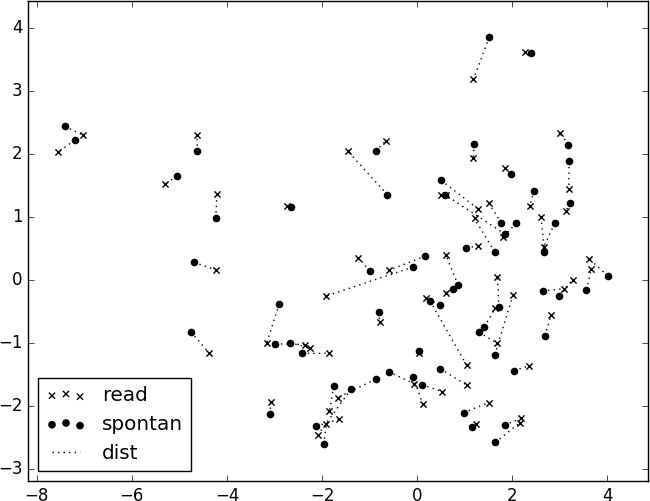
\includegraphics[width=3.25in]{perphon_dist1}
    \caption{Differences and positions of dictated-spontaneous phone pairs in 2-D space}
\label{phon_pca}
\end{figure}

\subsection{Segment Analysis}

General differences in spontaneous and dictated speech are observable from phoneme analysis.
Though useful for gaining insight as to why an existing model performs poorly, it is practical to be able to separate spontaneous and dictated speech in the absence of linguistic/grammatical information such as phones and (position in) words.
In the subsequent sections we shift the focus away from phones and the exploration of overarching differences between spontaneous and dictated speech, towards "anonymous" segments and the task of classifying spontaneous and dictated utterances. 

Based on insight from the analysis of phones in the previous section, a variation of the feature extraction pipeline is implemented whereby for each segment, in addition to the previous features, the difference in features against the preceding segment, henceforth "delta segments", are also extracted.
The purpose of these features is to embed local temporal information at the segment level.

To evaluate the feasibility of the feature set the segment data is first grouped into utterances and the average duration of spontaneous and dictated segments calculated.
The duration and intensity of spontaneous segments vary widely as compared to dictated speech; the standard deviation in duration and intensity in the examined corpus is an order of magnitude larger for spontaneous speech as compared to dictated.

As in the previous section, frame features are first averaged over segments using the full acoustic feature set described in the previous section.

The process is continued with bottom-up procedure.
Each ensemble in the system votes the label class.
This is done by choosing a class that has maximum support, total weight of classifiers that predict class $y$.
The voting rule is formalized by
\[\hat{y} = \argmax_y \sum_{c \in C \rightarrow y} w_c\]
where $\hat{y}$ is the ensemble result of label class, $C \rightarrow y$ is classifiers that predict $y$, and $w_c$ is the weight of the classifier.
And then, the result of each ensemble is combined to make one multilabel class of the document.

\begin{figure}[!htb]
\centering
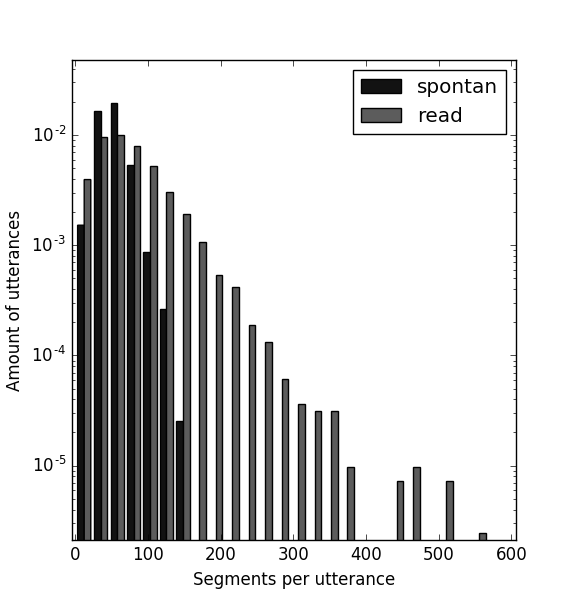
\includegraphics[width=3.2in]{nseg_per_utt_bw}
\caption{Number of members of each gender for each dialect}
\label{demographics1}
\end{figure}

\section{Utterance Classification}


\section{Results and Analysis}

\begin{figure}[!htb]
\centering
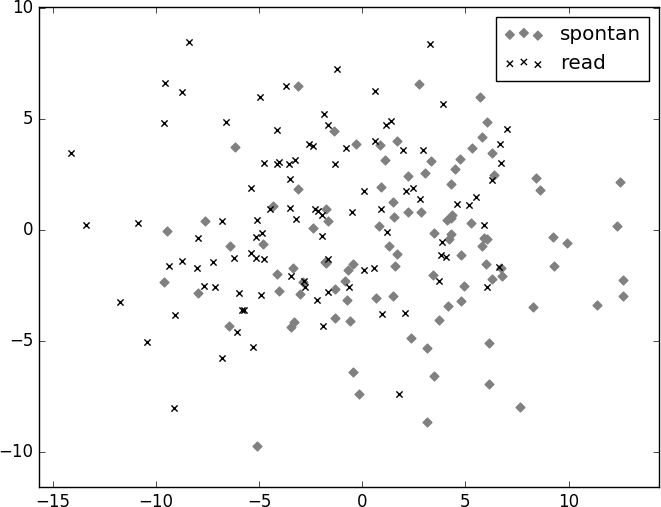
\includegraphics[width=3.2in]{pca}
\caption{Number of members of each gender for each dialect}
\label{demographics1}
\end{figure}

\begin{figure}[!htb]
\centering
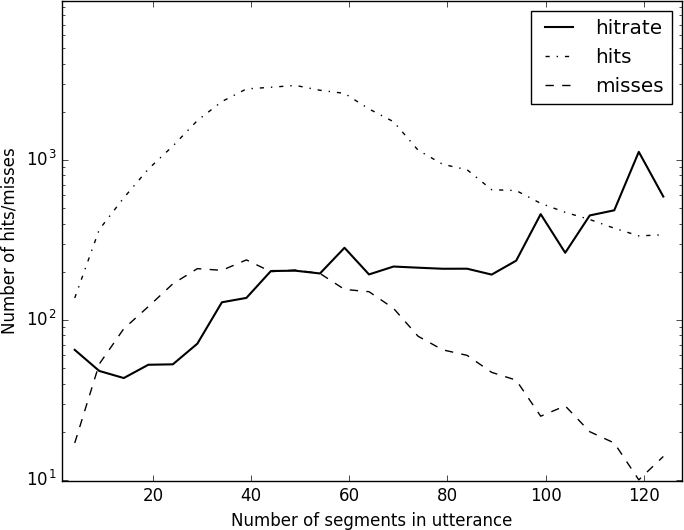
\includegraphics[width=3.2in]{hitrate}
\caption{Number of members of each gender for each dialect}
\label{demographics1}
\end{figure}

\section{Conclusion and further works}


\begin{thebibliography}{1}

\bibitem{laan}
G.P.M.~Laan,
    "The contributions of intonation, segmental durations, and spectral features to the perception of a spontaneous and a read speaking style,"
    Speech Communication 22:43-65, 1997.

\bibitem{dellwo}
V.~Delwo, A.~Leemann, M.J.~Kolly,
    "The recognition of read and spontaneous speech in local vernacular: The case of Zurich German,"
    Journal of Phonetics vol. 48, 2015, pp. 13-28.

\bibitem{silverman}
K.~Silverman, E.~Blaauw, J.~Spitz, J.~Pitrelli,
    "Towards Using Prosody in Speech Recognition/Understanding Systems: Differences Between Read and Spontaneous Speech",

\bibitem{liu}
G.~Liu, Y.~Lei, J.H.L.~Hansen,
    "Dialect Identification: Impact of Differences Between Read and Spontaneous Speech",
    18th European Signal Processing Conference (EUISPCO-2010), 2010.

\bibitem{furui1}
S.~Furui, M.~Nakamura, T.~Ichiba, K.~Iwano,
	"Why is the recognition of spontaneous speech so hard?",
	8th Internation Conference on Text, Speech, and Dialog,
	Karlovy Vary, 2005.

\bibitem{furui2}
S.~Furui,
    "Spontaneous Speech Recognition and Summarization",

\bibitem{benzeguiba}
M.~Benzeguiba, R.~DeMori, O.~Deroo, S.~Dupon, T.~Erbes, D.~Jouvet, L.~Fissore, P.~Laface, A.~Mertins, C.~Ris, R.~Rose, V.~Tyagi, C.~Wellekens,
	"Automatic Speech Recognition and Speech Variability: a Review",
	Speech Communication 49:763-786, 2007.

\bibitem{asami}
T.~Asami, R.~Masamura, H.~Masataki, S.~Sakauchi,
    "Read and spontaneous speech classification based on variance of GMM supervectors",
	Interspeech 2014:2375-2379, 2014.

\bibitem{nakamura2}
M.~Nakamura, I.~Koji, S.~Furui,
    "Differences between acoustic characteristics of spontaneous and read speech and their effects on speech recognition performance",
    Computer Speech and Language 22(2): 171-184, 2008.

\bibitem{sebastiani}
F.~Sebastiani,
    "Machine learning in automated text categorization,"
    ACM computing surveys (CSUR) 34.1 (2002): 1-47.

\bibitem{ayu}
A.~Purwarianti,
    "A non deterministic Indonesian stemmer,"
    Electrical Engineering and Informatics (ICEEI),
    2011 International Conference on. IEEE, 2011.

\bibitem{rahma}
D.~Rahmawati and M.L.~Khodra,
    "Automatic multilabel classification for Indonesian news articles,"
    Advanced Informatics: Concepts, Theory and Applications (ICAICTA),
    2015 2nd International Conference on. IEEE, 2015.

\bibitem{calandra}
R.~Calandra, et al.,
    "Learning deep belief networks from non-stationary streams,"
    Artificial Neural Networks and Machine Learning–ICANN 2012,
    Springer Berlin Heidelberg, 2012, 379-386.

\bibitem{muhlbaier}
M.D.~Muhlbaier and R.~Polikar,
    "An ensemble approach for incremental learning in nonstationary environments,"
    Multiple classifier systems, Springer Berlin Heidelberg, 2007, 490-500.

\bibitem{wang}
H.~Wang, F.~Wei, P.~Yu, and J.~Han,
    "Mining concept-drifting data streams using ensemble classifiers,"
    In Proceedings of the ninth ACM SIGKDD international conference on Knowledge discovery and data mining,
    pp. 226-235, ACM, 2003.

\bibitem{street}
W.~Street and Y.Kim,
    "A streaming ensemble algorithm (SEA) for large-scale classification,"
    Proceedings of the seventh ACM SIGKDD international conference on Knowledge discovery and data mining,
    ACM, 2001.

\bibitem{zang}
W.~Zang, et al.,
    "Comparative study between incremental and ensemble learning on data streams: case study."
    Journal Of Big Data 1.1 (2014): 1-16.

\bibitem{tsoumakas}
G.~Tsoumakas, I.~Katakis, and I.~Vlahavas,
    "Mining multi-label data,"
    in Data mining and knowledge discovery handbook,
    Springer, 2010, pp. 667–685.

\bibitem{prajapati}
P.~Prajapati, A.~Thakkar, and A.~Ganatra,
    "A Survey and Current Research Challenges in Multi-Label Classification Methods,"
    Int. J. Soft Comput., vol. 2, 2012.

\bibitem{demb}
K.~Dembczynski, W.~Waegeman, W.~Cheng, and E.~Hüllermeier,
    "On label dependence in multi-label classification,"
    in Workshop proceedings of learning from multi-label data,
    2010, pp. 5–12.

\bibitem{dharmadhikari}
S.C.~Dharmadhikari, M.~Ingle, and P.~Kulkarni,
    "A comparative analysis of supervised multi-label text classification methods,"
    2011.

\bibitem{zhang}
M.L.~Zhang and Z.H.~Zhou,
    "ML-KNN: A lazy learning approach to multi-label learning,"
    Pattern Recognit., vol. 40, no. 7, pp. 2038–2048, 2007.

\bibitem{santos}
A.~Santos, A.~Canuto, and A.~Neto,
    "A comparative analysis of classification methods to multi-label tasks in different application domains,"
    Int. J. Comput. Inform. Syst. Indust. Manag. Appl, vol. 3,
    pp. 218–227, 2011.

\bibitem{cherman}
E.A.~Cherman, M.C.~Monard, and J.~Metz,
    "Multi-label problem transformation methods: a case study,"
    CLEI Electron. J., vol. 14, no. 1, p. 4, 2011.

\bibitem{tala}
F.Z.~Tala,
    "A study of stemming effects on information retrieval in Bahasa Indonesia,"
    Institute for Logic, Language and Computation Universeit Van Amsterdam (2003).

\bibitem{sklearn}
F.~Pedregosa et al.,
    "Scikit-learn: Machine learning in Python,"
    The Journal of Machine Learning Research 12 (2011): 2825-2830.

\end{thebibliography}



% CONTEKAN:


% An example of a floating figure using the graphicx package.
% Note that \label must occur AFTER (or within) \caption.
% For figures, \caption should occur after the \includegraphics.
% Note that IEEEtran v1.7 and later has special internal code that
% is designed to preserve the operation of \label within \caption
% even when the captionsoff option is in effect. However, because
% of issues like this, it may be the safest practice to put all your
% \label just after \caption rather than within \caption{}.
%
% Reminder: the "draftcls" or "draftclsnofoot", not "draft", class
% option should be used if it is desired that the figures are to be
% displayed while in draft mode.
%
%\begin{figure}[!t]
%\centering
%\includegraphics[width=2.5in]{myfigure}
% where an .eps filename suffix will be assumed under latex, 
% and a .pdf suffix will be assumed for pdflatex; or what has been declared
% via \DeclareGraphicsExtensions.
%\caption{Simulation results for the network.}
%\label{fig_sim}
%\end{figure}

% Note that the IEEE typically puts floats only at the top, even when this
% results in a large percentage of a column being occupied by floats.


% An example of a double column floating figure using two subfigures.
% (The subfig.sty package must be loaded for this to work.)
% The subfigure \label commands are set within each subfloat command,
% and the \label for the overall figure must come after \caption.
% \hfil is used as a separator to get equal spacing.
% Watch out that the combined width of all the subfigures on a 
% line do not exceed the text width or a line break will occur.
%
%\begin{figure*}[!t]
%\centering
%\subfloat[Case I]{\includegraphics[width=2.5in]{box}%
%\label{fig_first_case}}
%\hfil
%\subfloat[Case II]{\includegraphics[width=2.5in]{box}%
%\label{fig_second_case}}
%\caption{Simulation results for the network.}
%\label{fig_sim}
%\end{figure*}
%
% Note that often IEEE papers with subfigures do not employ subfigure
% captions (using the optional argument to \subfloat[]), but instead will
% reference/describe all of them (a), (b), etc., within the main caption.
% Be aware that for subfig.sty to generate the (a), (b), etc., subfigure
% labels, the optional argument to \subfloat must be present. If a
% subcaption is not desired, just leave its contents blank,
% e.g., \subfloat[].


% An example of a floating table. Note that, for IEEE style tables, the
% \caption command should come BEFORE the table and, given that table
% captions serve much like titles, are usually capitalized except for words
% such as a, an, and, as, at, but, by, for, in, nor, of, on, or, the, to
% and up, which are usually not capitalized unless they are the first or
% last word of the caption. Table text will default to \footnotesize as
% the IEEE normally uses this smaller font for tables.
% The \label must come after \caption as always.
%
%\begin{table}[!t]
%% increase table row spacing, adjust to taste
%\renewcommand{\arraystretch}{1.3}
% if using array.sty, it might be a good idea to tweak the value of
% \extrarowheight as needed to properly center the text within the cells
%\caption{An Example of a Table}
%\label{table_example}
%\centering
%% Some packages, such as MDW tools, offer better commands for making tables
%% than the plain LaTeX2e tabular which is used here.
%\begin{tabular}{|c||c|}
%\hline
%One & Two\\
%\hline
%Three & Four\\
%\hline
%\end{tabular}
%\end{table}


% Note that the IEEE does not put floats in the very first column
% - or typically anywhere on the first page for that matter. Also,
% in-text middle ("here") positioning is typically not used, but it
% is allowed and encouraged for Computer Society conferences (but
% not Computer Society journals). Most IEEE journals/conferences use
% top floats exclusively. 
% Note that, LaTeX2e, unlike IEEE journals/conferences, places
% footnotes above bottom floats. This can be corrected via the
% \fnbelowfloat command of the stfloats package.



% trigger a \newpage just before the given reference
% number - used to balance the columns on the last page
% adjust value as needed - may need to be readjusted if
% the document is modified later
%\IEEEtriggeratref{8}
% The "triggered" command can be changed if desired:
%\IEEEtriggercmd{\enlargethispage{-5in}}



% that's all folks
\end{document}

